%!TEX root = Memoria_TFM.tex
%\minitoc
%\mtcskip
\begin{small}
\emph{In this chapter the evolution of the built Convolutional Neural Network architecture, the experiments carried out and its corresponding results, are described.}
\end{small}

\section{LeNet-5}
LeNet-5 \cite{Lenet5} is the name of a certain architecture of a convolutional network designed for document recognition (handwritten, machine printed characters) developed by Yan Lecun \textit{et al}.\\

\begin{figure}[htb]
  \centering
  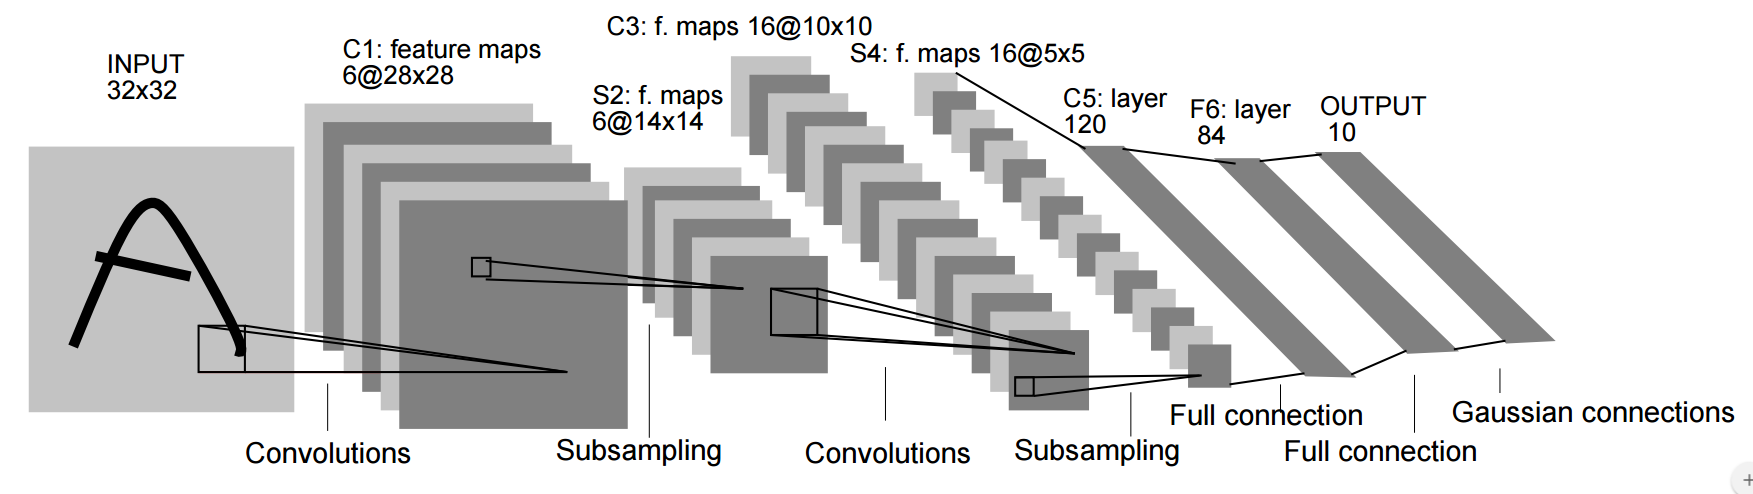
\includegraphics[width=0.7\textwidth]{images/images_lenet/LenetArquitectura.png}
  \caption{LeNet-5 Arquitecture.}
  \label{Lenet5Arquitectura}
\end{figure}

The basic architecture of LeNet-5 is two convolutional layers, each one of them followed by a max pooling layer and then a fully-connected layer. This architecture could be visualized in figure \ref{Lenet5Arquitectura} where it is possible to visualize the input image dimensions across the layers and its final shape.\\

LeNet is a useful convolutional neural network that is usually used by beginner users to learn deep learning matters due to its short architecture and because it is implemented in many deep learning frameworks using it to explain the framework. Because of this, LeNet-5 has been used as the basis of the project and to learn the Theano implementation and the Convolutional Neural Networks theory.\\

The code of LeNet in Python using the Theano library, and its explanation, is openly available in \url{www.deeplearning.net}.

\subsection{LeNet-5 specifications}
The architecture of the LeNet-5 downloaded code, used to start working in this project, is formed by two convolutional layers (size 5x5) with 20 kernels in the first convolutional layer and 50 in the second one. Each one of these followed by a max pooling-layer of size 2x2. Those four layers are followed by a fully-connected layer with 500 neurons at the output.\\

The classifier, which has been used is the logistic regression, has indeed been at the same time as the Convolutional Neural Network. The activation function of the convolutional layers and the logistic regression is the hyperbolic tangent (tanh). The learning rate used is 0.1 and the network runs by 200 epoch.\\

The cost function, or loss that must be minimized during the training, is the negative log-likelihood. LeNet-5 uses the stochastic gradient method with mini-batches (MSGD).\\

The data used is MNIST digit database, whose characteristics are described in section \ref{subsec:MNIST}. The data consists of three subsets: training, testing and validating. Each subset is used for training, testing or validating, respectively.\\

The data is not fed to the network all at once, each subset is grouped in small subsets called batches and whose size is chosen by the user.In the code available of LeNet-5 the batch size is 500 samples. The network is fed by batches, so the size of the net depends on the batch size not the (train, test or validate) subset. In this example, the batch size, is the same for the three subsets. When the subset is divided into different batches, if there are samples that are not enough for a batch, those samples are not used.\\

The network train for a specified number of epoch. Each epoch has as many iterations as necessary to go through all batches of the train subset. The reason for using batches is to define the size of the network and because, usually, the quantity of samples used in deep learning is large (thousand, millions..) and too much memory would be needed to build a network of its size and the computational resources available may not be enough.\\

As the MNIST digit database available with the code has 50000 samples for training, 10000 for testing and 10000 for validating, the number of batches for each subset (with 500 samples for each batch) is 100 for training, 20 for testing and 20 for validating

The training procedure is being carried out for too many epochs as user has selected and returned the cost of the procedure. While the training is running, the validation is calculated for each epoch and the validation returns the error of the procedure. The training cost and the validation error are used to know the behaviour or the learning process of the network and how it generalizes with the purpose of choosing the best model.\\

The test is realized while the training is being executed, more specifically, when the validation has been done and the best results have been obtained during the whole process until that iteration. The result that is used to compare with others classifiers or with others articles.\\

In addition to the number of epochs, an alternative approach would be to stop the training procedure (\textit{early-stopping}). This method is used to avoid over fitting tracking the validation process \cite{Yoshua}. decision to stop the training depends on \textit{the patience}. User chooses \textit{patience} value.

%%%%% Creo que esto de aqui abajo no es necesario %%%%%%
%First of all in Lenet the data is loaded. The function that download the data check, firstly, if the data is not downloaded yet, if it downloaded it does not repeat the download. The data is downloaded split into train, test and validation subsets.\\

%After loading the data, the architecture is defined, the layers are called because they has been defined as objects, each kind of layer, one different object. There is a object for convolutional + maxpooling, another object for the hidden layers that is a fully connected layer, and the classifier used that is logistic regression. Each part of the code could be found in \url{www.deeplearning.net}\\

%After creating the structure, the functions of training, validating and testing are created as Theano functions.\\

%In a big while loop the training validation and testing is developed. The data is trained. Each mini-batch (that is a small quantity of that given by the user, it is used in order to not train or test all the data together because it would take too much computer resources) is trained and the weights and bias of each layer are updated. It is given a validation frequency, this parameters decides how many validations are produced. So the data is trained and validation, when a best score of validation is produced, the data is tested.\\

%The training would run for a number of epoch that the user has given or by a early-Stopping that has been developed by authors. The early-stopping combats over-fitting by monitoring the model's performance on a validation set.\\

\subsection{LeNet-5 Results} \label{sec:lenet_results}
While the training is being calculated, the weights are being updated in each iteration. When a  model is selected or saved, weights are indeed what is being chosen or saved. An example of weights is represented in figure \ref{fig:weights_lenet} where twenty first weights at epoch 10 of the first convolutional layer are demonstrated. Therefore when it is being trained, what the network is doing is adapting the weights to the input to get a good performance.\\

\begin{figure}[htb]
\centering
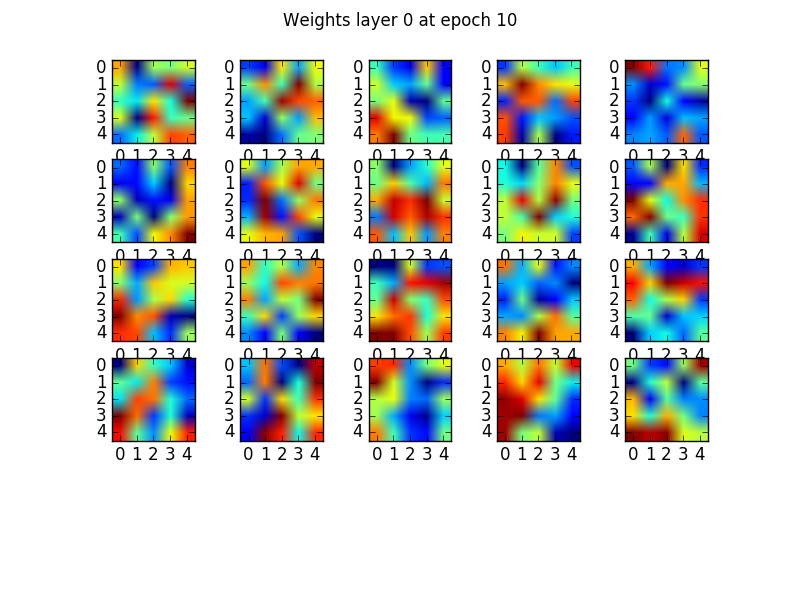
\includegraphics[width=0.7\textwidth]{images/images_lenet/w_layer0_epoch10.png}
\caption{Weights at epoch 10 of the first convolutional layer.} \label{fig:weights_lenet}
\end{figure}

The training procedure returns the cost function in each iteration to evaluate the training behavior. The cost function obtained at training by  executing LeNet-5 is represented in figure \ref{fig:Lenetcost}, and its value decreases as the iterations rise converging in almost 0; this curve is the desired one for each training practice, as it is does not oscillate abruptly and converges in a very low value logarithmically.\\

\begin{figure}[htb]
\centering
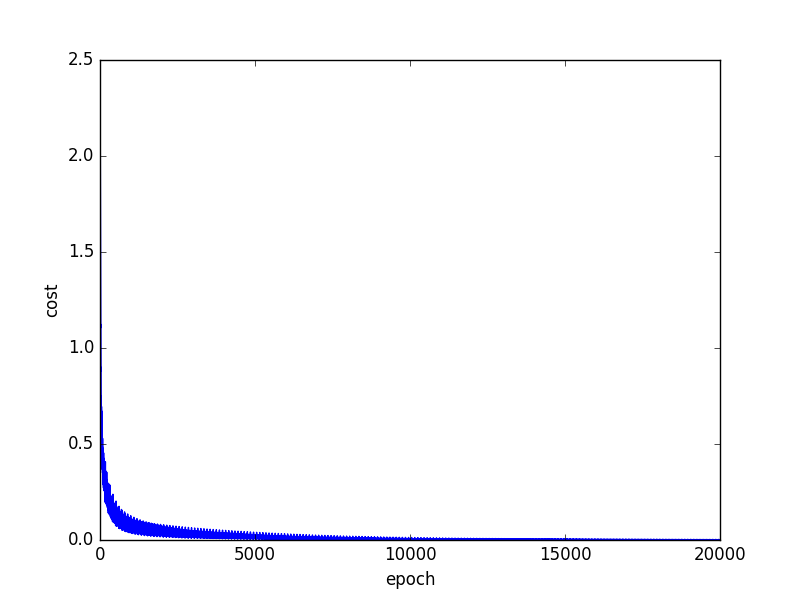
\includegraphics[width=0.7\textwidth]{images/images_lenet/cost_lenet.png}
\caption{Cost function at training running LeNet-5 with MNIST digit database.} \label{fig:Lenetcost}
\end{figure}

The error obtained at validation is represented in figure \ref{fig:Lenetresult}, where it could be seen that the value decreases logarithmically to converge, approximately, in 1 (a low value) and this behavior of the curve is the desired one in a validation process. The convergence value of the validation is not usually as low as the training convergence value, and the point where it starts to converge is at a subsequence later than in the training.\\

\begin{figure}[htb]
\centering
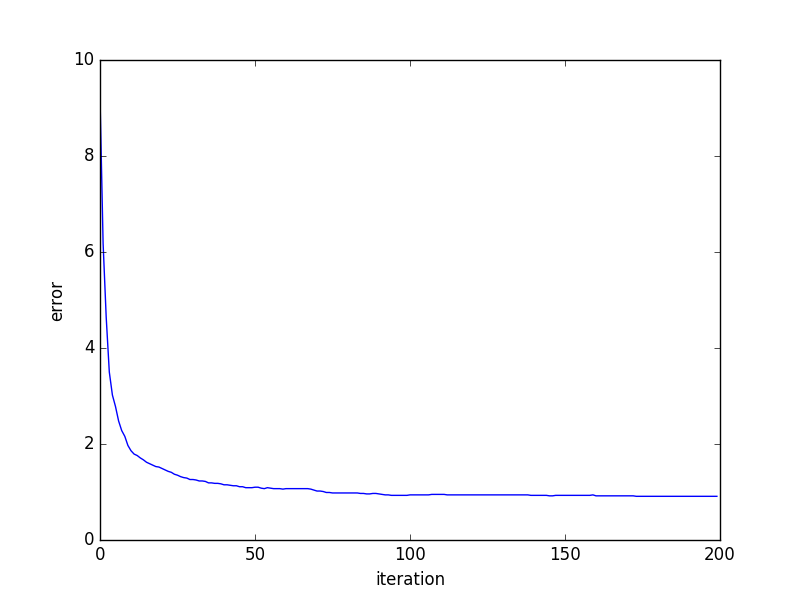
\includegraphics[width=0.7\textwidth]{images/ModificandoLenet/error_lenet.png}
\caption{Validation error obtained with LeNet-5 with MNIST digit database.} \label{fig:Lenetresult}
\end{figure}

The test result has been calculated with the model acquired in iteration 18300 (epoch $37^{th}$), with a validation error of 0.91\%. The error rate obtained is 0.92\% which means that 920 samples out of 100000 of the testing subset are being misclassified.

%The neural network has beoen built in Python using Theano library. The %network has been based on the one exposed in \textit{Learn Convolutional %Neural Network for Face Anti-Spoofing} and \textit{LeNet}.\\
%The architecture of the network is formed by two convolutional layers which %is followed (each one) by a max-pool layer.The  last max-pool layer is %followed by a fully-connected layer which have sigmoidal activation %function.\\
%The rectified linear activation function (reLu) is used as activation %function of the convolutional layers. It has been used a normalized %distribution of weights and bias, the same which was implemented in LeNet: %weights are sampled randomly from a uniform distribution in the range [-1/%fan-in, 1/fan-in], where fan-in is the number of inputs of the previous %layer. The ReLu function that has been used is the one implemented in %theano as theano.tensor.nnet.relu.\\
%The number of kernels used in the conv layers are 48 and 96 of size 5x5, %the size of the max-pool layer is 2x2.\\
%The network is trained with the 70\% of the data, the 30\% is used to test. %From the 70\% of the training data, the 25\% is used to validation.\\

\subsection{Modifying LeNet}
Modifications have been made to LeNet-5 architecture. Firstly, the batch size has been changed. Then the tanh activation function has been replaced, a normalization layer has been added and the weight initialization has been changed too. The database used for these experiments is the MNIST digit database.

\subsubsection{Changing the batch size}
Two experiments have been developed in order to compare the results when the batch size is changed and how the network behaviour changes too with regard to LeNet-5 with the original batch size (500).\\

The first experiment contained 20 samples per batch. For the second experiment, the batch size used is 100. In both cases, the training process was stopped by the early-stopping; at epoch $31^{th}$ it stopped the first experiment, because from the epoch $16^{th}$ epoch the error at validating was not improving and for the second experiment, at $33^{th}$ epoch, the early-stopping finished the training.\\

The validation error for both experiments and the original LeNet are represented in figure \ref{figures:LENET-batches}. From the images it could be seen that the validation error in first epochs is lower (9 \% in the first experiment) than the validation error when the batch size is bigger. When the batch size is equal to 20, the optimal test error rate is obtained in the first $15^{th}$ epochs, the same error rate than in the original case (0.92\%). However for 100 samples per batch, it has not been possible to get to that error rate, the best test error rate has been 1.04\% at iteration 8500.\\

\begin{figure}[htb]
    \centering
	\subfigure[batch size = 500 (original size)]{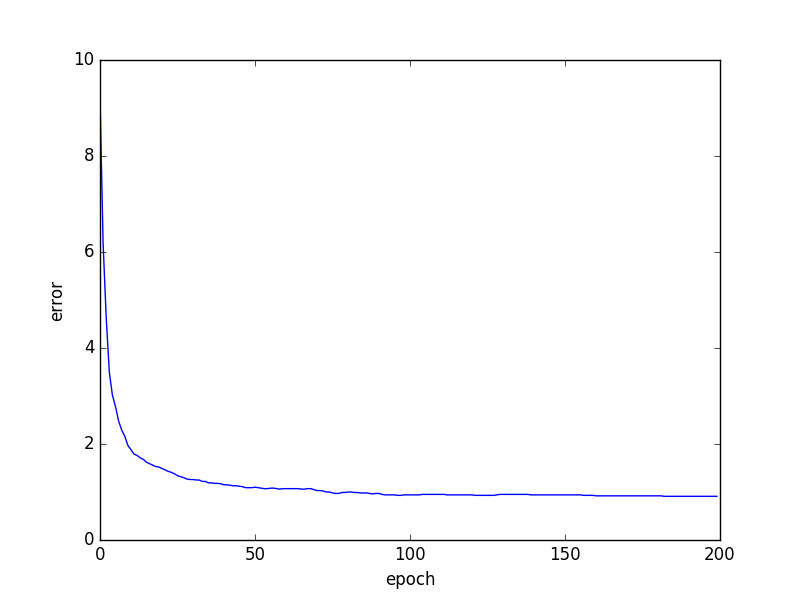
\includegraphics[width=0.47\textwidth]{images/images_lenet/lenet_batch/lenet_500batch_rror.png} }
	\subfigure[batch size = 20]{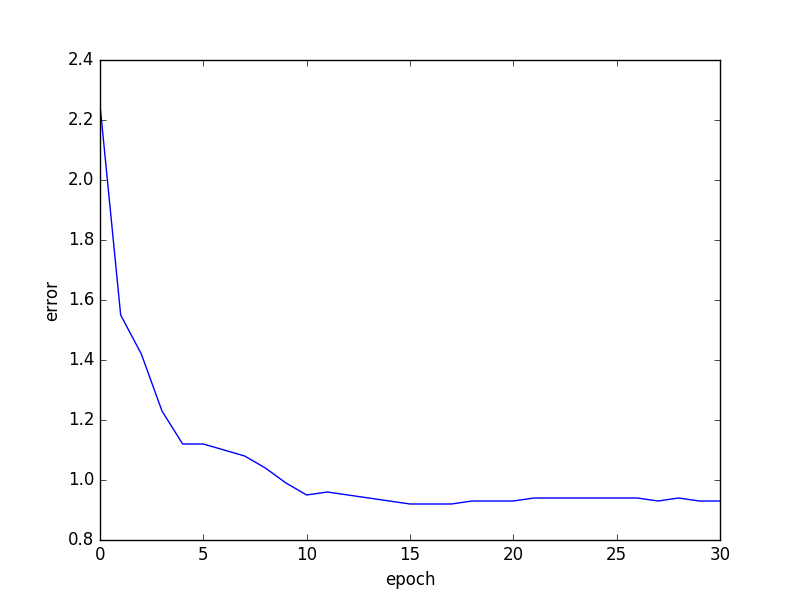
\includegraphics[width=0.47\textwidth]{images/images_lenet/lenet_batch/lenet_20batch_error.png} }
	\subfigure[batch size = 100]{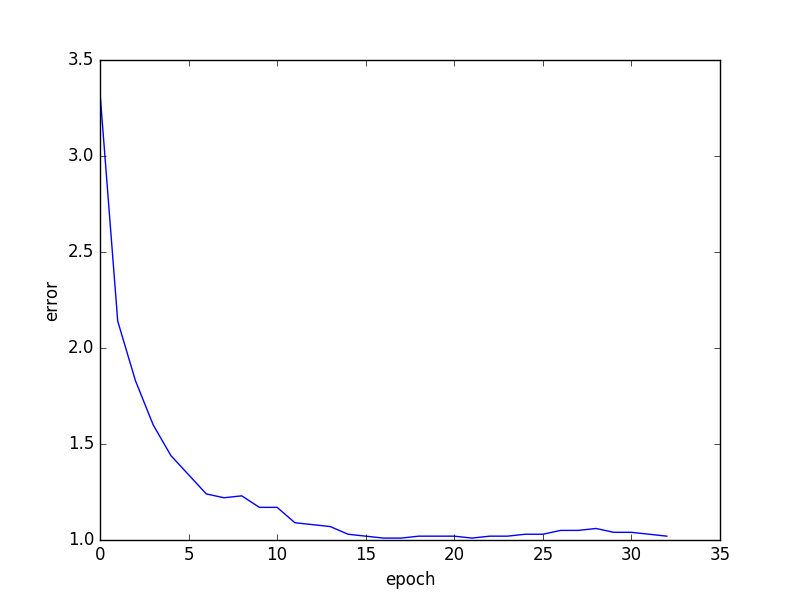
\includegraphics[width=0.47\textwidth]{images/images_lenet/lenet_batch/lenet_100batch_error.png} }

    \caption{Validation error in each epoch for different sizes of batches.} \label{figures:LENET-batches}
\end{figure}

%Each time we take a sample and update our weights it is called a mini-batch. Each time we run through the entire database, it's called an epoch. Batch size determines how many examples you look at before making a weight update. The lower it is, the noisier the training signal is going to be, the higher it is, the longer it will take to compute the gradient for each step. \url{http://stats.stackexchange.com/questions/140811/how-large-should-the-batch-size-be-for-stochastic-gradient-descent}.\\

To conclude, more epochs are necessary when the batch size is bigger, because there are not enough updates in each epoch \cite{Yoshua}. Usually, the value of the batch size used is 32 \cite{Yoshua} and generally, the choice is computational.\\

In figure \ref{figures:LENET-batches} the error in each epoch is represented  with a batch size of 500, the original size, 20 and 100. In the original case, the error starts with a value of 9\% approx. When the batch size equals 20, the error in the first iteration is about 2.4\%. Finally, with a batch of 100 images, the validation error is 3.5\%.\\

With the original size and size equal to 20, it is possible to get to the same minimum error, the difference between those examples is that each one gets to that conclusion into different epochs. With a batch size equal to 100, the code stopped in epoch 33 because of the early-stop with a patience of 10000 obtaining a 1.04\% test error at iteration 8500 and a 1.01\% validation error. With a batch size equal to 20, the code also  stopped earlier because of the same reason. Nonetheless, in this case it was possible to get to the same minimum as with the original size: the epoch in which it stopped was 31, it ran without getting a better validation score for 15 epochs.

%If the patience is increased from 10000 to 100000 for a batch size = 20 and equal to 100, results obtained are that for a value of 20, it has been running for 40 epoch, having the same results that the one obtained with a patience of 10000.\\
%For a value of 100 with the patience increased to 100000, the results are not the same as the one obtained the patience equal to 10000. In this occasion, the results are better than in the original one; The code has run for 258,08 minutes and for 200 epochs. The result obtained was better than in the original one has it has said. In epoch 51 has gotten a validation error of  1 \% and the error test has been 0,89\%, from this point, the test error that has been calculated five more times, has been increasing until get the value 0,85\% in iteration 55500, epoch number 111, the validation error obtained has been 0,95\%. From this epoch until number 200, the network has not had any better result.\\
%In figure X it is possible to see the error function for those two examples. It could be seen that the example with batch size = 20 has just run for 40 epoch and the good results of the example with batch size = 100, remembering that the patience has been increased from 10000 to 100000.\\

\subsubsection{Changing the activation function, normalization and weights initialization}
Just as the batch was changed and its results were compared in the previous subsection, the activation function has also been changed, a normalization layer has been added and weights initialization has been changed.\\

LeNet-5 does not use any normalization layer, but in this experiment from the different normalization availables (batch normalization, local normalization, etc.) Local Response normalization is added after the max-pooling layers.\\

The activation function used in LeNet-5 is tanh (hyperbolic tangent), it has been substituted to rectified linear unit (ReLu) activation function.\\

Regarding the weight initialization, in LeNet, for the convolutional layers and the fully connected layer,  a normalized initialization \cite{XavierInitialization} is used:

\begin{equation}
  W \sim U [- \frac{\sqrt{6}}{\sqrt{n_{j}+n_{j+1}}},\frac{\sqrt{6}}{\sqrt{n_{j}+n_{j+1}}}]
\end{equation}

Where $n_{j}$ is the number of neuron of the current layer and $n_{j+1}$ is number of neurons of the following layers. In this experiment, this initialization has been changed to a weight initialization with a Gaussian distribution.\\

Here below the details of each experiment are described:
\begin{itemize}
\item{Experiment 1: using Local Response Normalization (LRN) In which a normalization has been carried out in the convolutional-max pooling layers.}
\item{Experiment 2: using ReLu as activation function:} The activation function tanh has been substituted by ReLu activation function in convolutional and fully connected layers.
\item{Experiment 3: using ReLu and LRN}: The activation function used is ReLu and LRN has been used as  normalization layer.
\item{Experiment 4: changing weights initialization}: Weights initialization has been changed by Gaussian. In which the mean value that has been used is 0 and std is 0.01. Weights initialization has been changed in convolutional and fully connected layers. Also, bias initialization has been changed by ones.
\end{itemize}

%Using Local Response Normalization we want to detect high frequency features with a large response. If we normalize around the local neighborhood of the excited neuron, it becomes even more sensitive as compared to its neighbors.[\url{https://prateekvjoshi.com/2016/04/05/what-is-local-response-normalization-in-convolutional-neural-networks/}].\\

In figure \ref{fig:LenetModifications} what is represented is the cost at training (figure \ref{fig:cost_lenet_modifications}) and the error at validation (figure \ref{fig:error_lenet_modifications}) of the four training process experiments  with the original LeNet-5 results. Each network has run 200 epoch, except when early-stopping was needed.
\begin{figure}[tb]    \centering
	\subfigure[Cost at training]{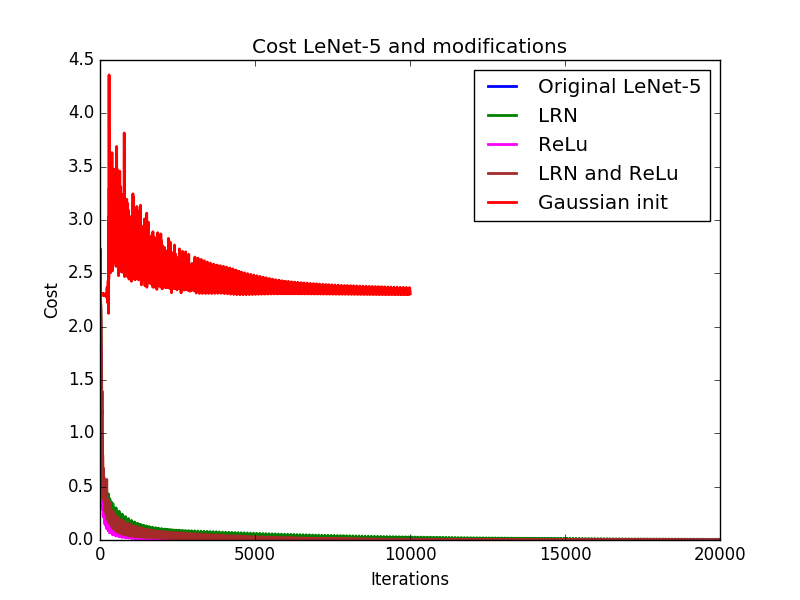
\includegraphics[width=0.48\textwidth]{images/ModificandoLenet/Cost_Lenet5_modifications.png}\label{fig:cost_lenet_modifications} }
	\subfigure[Error at validation]{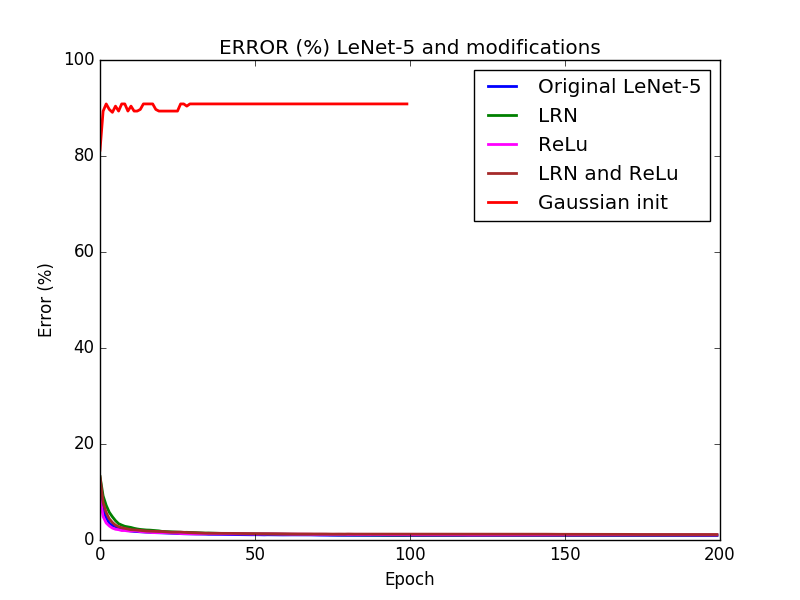
\includegraphics[width=0.48\textwidth]{images/ModificandoLenet/Error_Lenet5_modifications.png}\label{fig:error_lenet_modifications}}
    \caption{Cost at training and error at validatioin of LeNet-5 and the four experiments.} \label{fig:LenetModifications}
\end{figure}

From figure \ref{fig:LenetModifications}, the first observation is that the Gaussian initialization has worsened the original result significantly, the cost converges in 2.3 while in other experiments it converges in a value close to 0; therefore, the training has converged in a local minimum. Moreover, the early-stopping led the training process for the fourth experiment Gaussian initialization experiment) to stop in $100^{th}$ epoch.\\

From figure \ref{fig:LenetModifications},  it can also be deduced that the training and validation processes in other experiments' behaviour is similar to the original LeNet-5 performance.\\


The results obtained at validation and testing for each experiment are exposed in table \ref{Experiments-lenet}.

\begin{table}[tb]
\centering
\resizebox{0.95\textwidth}{!}{%
\begin{tabular}{|c|c|c|c|}
\hline
\rowcolor[HTML]{ECF4FF}
{\color[HTML]{333333} \textbf{CNN model}} & {\color[HTML]{333333} \textbf{Description}} & {\color[HTML]{333333} \textbf{Best validation Error}} & {\color[HTML]{333333} \textbf{Test Error}} \\ \hline
Lenet-5       &     Original Lenet-5 without modifications  &              0.91\% (17400 iter.)              &                         0.92\%             \\ \hline
Experiment 1  &    Using Local Response Normalization       &              0.99\%  (13400 iter.)             &                          1.6\%            \\ \hline
Experiment 2  &    Using ReLu as activation function        &              1.04\% (11900 iter.)              &                          2.4\%            \\ \hline
Experiment 3  &     Using ReLu and LRN                      &              1.18\%   (19500 iter.)             &                          1.08\%          \\ \hline
Experiment 4  &     Gaussian weight initialization          &              81.22\%  (100 iter.)              &                          80.90\%         \\ \hline
\end{tabular}%
}
\caption{Lenet-5 experiments results.}
\label{Experiments-lenet}
\end{table}

From table \ref{Experiments-lenet}, it could be concluded that the best configuration for the network is the original one. With Gaussian initialization, the network does not find a local minimum in such time. Using LRN and ReLu, the test result is closer to the one obtained with the original LeNet-5, but not as good as the last one. Changing the activation function has not been a good change. Not taking into account the original LeNet-5, the best test performance has been obtained with 1,08\% using ReLu and LRN, but the best validation error is 0,99\% obtained using just LRN. The modifications results are similar, except in experiment 4.

\subsection{LeNet-5 and RGB FRAV faces database} \label{Lenet-FRAV}
The objective of this thesis is to train a convolutional neural network for face anti-spoofing, for which the following step is to feed LeNet-5 with a face database, RGB FRAV database.\\

In order to work with images, because of the difference among the shape of the images, they have been resized into 252x180. This new shape is proportional to $0.7*height = weight$ because all studied images save that proportion approximately.\\

The network has been tested with this database in the two ways to classify images: with two classes (genuine and attacks) and five classes (genuine and four classes, one per type of attack).\\

The architecture used is the same as LeNet-5 except for the batch size that has been reduced to 50 because there are not as many samples as in the MNIST database.\\

\begin{figure}[tb]
\centering
\subfigure[Cost]{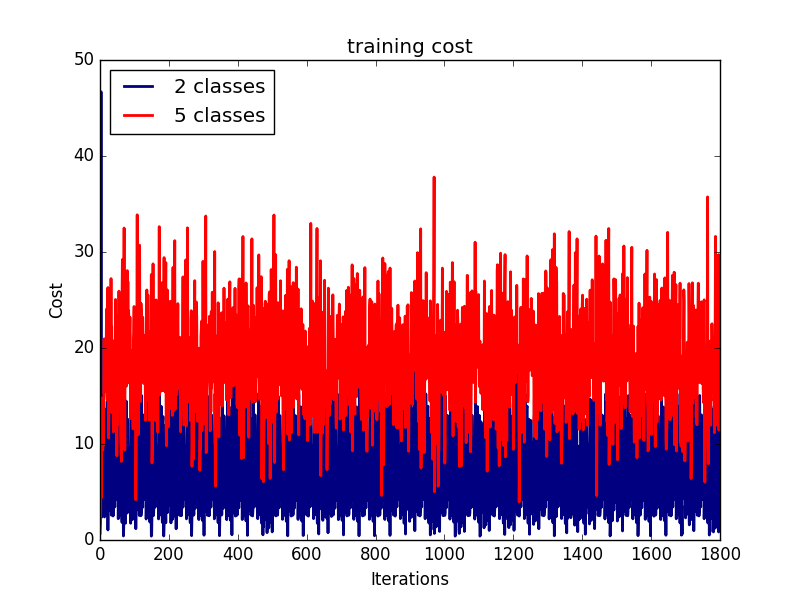
\includegraphics[width=0.47\textwidth]{images/ModificandoLenet/lenet_frav_cost.png}\label{Lenet_FRAV_cost} }
\subfigure[Error]{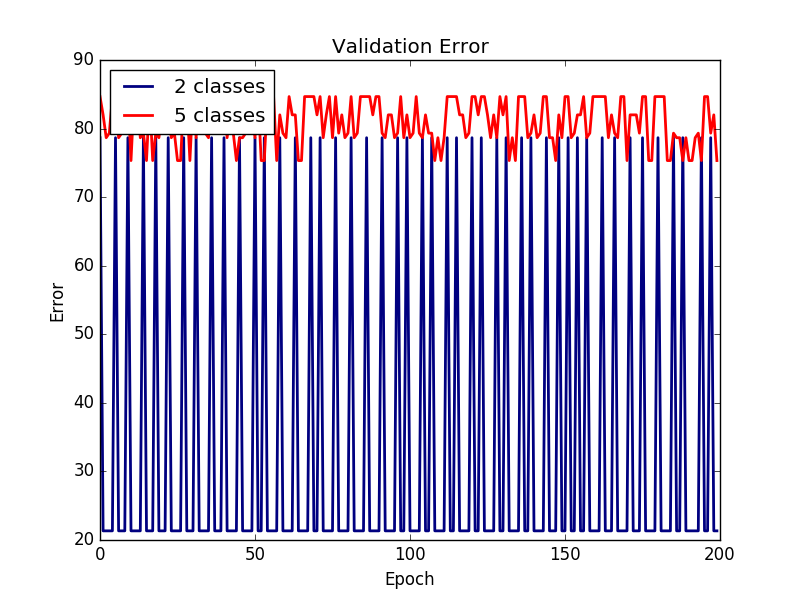
\includegraphics[width=0.47\textwidth]{images/ModificandoLenet/lenet_frav_error.png} \label{Lenet_FRAV_error} }
\caption{Cost at training (a) and Error at validation (b) when LeNet has been used with RGB FRAV database.}
\label{fig:Lenet_FRAV}
\end{figure}

Figure \ref{fig:Lenet_FRAV} represents the training cost \ref{Lenet_FRAV_cost} and the validation error \ref{Lenet_FRAV_error} of the training process. In the figure, it is represented in blue when 2 classes are used to classify and red when 5 classes are used, for both cases (cost and error). From the figure it is possible to visualize that the whole training process is not desirable for 2 classes and 5 classes, because it seems that the network does not learn, the architecture requires to be modified.


\section{Adapting LeNet-5 architecture} \label{sec:adapt_lenet}
From LeNet-5 architecture, changes have been made in order to build a similar convolutional architecture as described in \cite{yangLL14}. LeNet-5 architecture is simple to use  for this project’s purpose.\\

In \cite{yangLL14} authors develop a convolutional neural network with similar objectives as the one described in this thesis. The CNN is based on \textit{Imagenet} architecture \cite{imagenet}, this is a specific architecture used to classify objects which are well known and regularly used in the deep learning community. Its architecture is described in figure \ref{fig:Imagenet_architecture}.\\

\begin{figure}[tb]
\centering
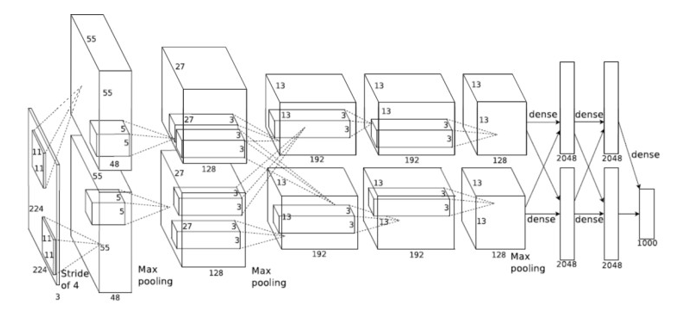
\includegraphics[width=0.75\textwidth]{images_miscelaneus/Imagenet.png}
\caption{Imagenet architecture.} \label{fig:Imagenet_architecture}
\end{figure}

Imagenet is formed by convolutional layers, max-pooling layers, normalization layers, dropout layers and a fully-connected layer.\\

Authors from \cite{yangLL14} slightly describe the architecture, the parameters and the changes made from Imagenet. Therefore, it is not possible to develop an architecture based on the one used in the article \cite{yangLL14}, hence, it is going to be based on Imagenet.\\

%Dentro de la carpeta de FRAv\_casia\_ImageNet, en imagenet2, se ha programado imagenet, lo unico que sin strides en la primera capa de convolucion.\\
%Because of the lack of information about the convolutional neural network described in casia paper, it has been necessary  to though the original code that authors use, Imagenet. Authors use the same architecture, although how it has been modified it is not explained. \\
%It has been possible to implement Imagenet, the difference between the implementation and the original one is that the strides used in the first convolutional layer has not been used because the input of the images need to be bigger to have more than one neuron in the last layer.\\
%Dentro hay una carpeta para cada base de datos. Dentro de cada carpeta estan las pruebas que se hacen con cada base de datos.\\
%The convolutional neural network has been tested with different databases: FRAV, CASIA and MFSD and different experiments have been carried out with each one.\\
\subsection{New Architecture} \label{subsec:ejecucion1}
%Ejecucuion1
The new architecture comprises the following layers:
\begin{itemize}[itemsep=2pt,topsep=8pt,parsep=0pt,partopsep=20pt]
\item Convolutional layer with 96 kernels of size 11x11 followed by a max-pool layer (2x2 size) and a local response normalization.
\item Convolutional layer with 256 kernels whose size is 4x4.
\item Convolutional layer with 386 kernels whose size is 3x3.
\item Convolutional layer with 384 kernels whose size is 3x3.
\item Convolutional layer with 256 kernels whose size is 3x3 followed by a max-pool layer of 2x2 size.
\item Dropout layer with 4096 neurons.
\item Dropout layer with 4096 neurons.
\item Fully Connected layer with 2000 neurons at the output.
\end{itemize}

ReLu has been used as an activation function. Logistic regression has been used in the training process. Weights have been initialized with Gaussian initialization and bias to 1. The learning rate value is 0.01.

\subsection{Databases} \label{subssec:ejec1_database}
The databases used in for experiments are CASIA images, CASIA videos, RGB FRAV, (RGB+NIR) FRAV feature level database and MFSD-MSU database. Just two classes are going to be used in this experiment: class 0 is real users class and class 1 is attack class.\\

Samples distribution are described in table \ref{Samples_distribution} where the number of samples per class and  subset (train, test and validation) are summarized for each database. It is possible to realize that the number of positive (class 0) samples is lower for all the databases, but more specifically, the amount of positive samples in MFSD-MSU database is very small.\\

\begin{table}[htb]
\centering
\begin{tabular}{c|c|c|c|c|c|}
\cline{2-6}
                       & \cellcolor[HTML]{ECF4FF}\begin{tabular}[c]{@{}l@{}}RGB\\ FRAV\end{tabular} & \cellcolor[HTML]{ECF4FF}\begin{tabular}[c]{@{}l@{}}RGB+NIR\\ FRAV\end{tabular} & \cellcolor[HTML]{ECF4FF}\begin{tabular}[c]{@{}l@{}}Images\\ CASIA\end{tabular} & \cellcolor[HTML]{ECF4FF}\begin{tabular}[c]{@{}l@{}}Videos\\ CASIA\end{tabular} & \cellcolor[HTML]{ECF4FF}MFSD-MSU \\ \hline

\multicolumn{1}{|c|}{\cellcolor[HTML]{ECF4FF}Train samples class 0} & 157                              & 133                                    & 26                                   & 255                                  & 30                           \\ \hline
\multicolumn{1}{|c|}{\cellcolor[HTML]{ECF4FF}Train samples class 1} & 459                              & 417                                    & 111                                  & 81                                   & 68                           \\ \hline \hline
\multicolumn{1}{|c|}{\cellcolor[HTML]{ECF4FF}Valid samples class 0} & 10                               & 8                                      & 7                                    & 105                                  & 2                            \\ \hline
\multicolumn{1}{|c|}{\cellcolor[HTML]{ECF4FF}Valid samples class 1} & 83                               & 70                                     & 13                                   & 39                                   & 12                           \\ \hline \hline
\multicolumn{1}{|c|}{\cellcolor[HTML]{ECF4FF}Test samples class 0}  & 19                               & 16                                     & 16                                   & 540                                  & 3                            \\ \hline
\multicolumn{1}{|c|}{\cellcolor[HTML]{ECF4FF}Test samples class 1}  & 167                              & 70                                     & 23                                   & 180                                  & 25                           \\ \hline
\end{tabular}\caption{Samples distribution for each database.}
\label{Samples_distribution}
\end{table}

Databases are built independently of the CNN process. Images are read, shuffled and splited in train, test and validation subsets in order to be saved in a pickle file and used in the same way as much times as necessary without being reading the raw data.

\subsection{Experiments Description} \label{sec:experiments_ejec1}
With that databases. Some experiments has been carried out. To test, the used classifier is SVM with RBF, the parameter \textit{C} has been searched for each experiment:
\begin{itemize}
\item General experiment: the architecture described in \ref{subsec:ejecucion1} is trained without changes.
\item Experiment 2: with the purpose of trying to know if the configuration of the network is correct, only it is going to be trained with 20 samples for each subset, expect for MFSD-MSU database in which 14 samples are used.
\item Experiment 3: with the purpose of provoke overfitting, 20 samples are used for each subset, however validation samples are the same as training samples.
\item Experiment 4: the finality is the same as Experiment 3, knowing the behaviour of the network and provoke overfitting, but differs in the learning rate that has been changed to 0.001 value. \\
\end{itemize}

%Experiment 2 and experiment 3 would have the same training cost curve, because they differs in the validation subset.\\

Because the training process in experiment 2 and experiment 3 should be the same (the difference among those experiments is the validation process, and thus test process), only one cost would be represented.\\

In figures \ref{fig:casia-ejec1}, \ref{fig:casiavid-ejec1}, \ref{fig:frav-ejec1}, \ref{fig:frav_imagelevel-ejec1}, \ref{fig:frav_classlevel-ejec1} and \ref{fig:mfsd-ejec1} are represented the cost at training and the error at validation, for each database, when the four described experiments have been developed. All figures have the same color legend which is summarized in table \ref{table:color_legend}.\\

\begin{table}[htb]
\centering
\begin{tabular}{|c|c|}
\hline
\rowcolor[HTML]{ECF4FF}
\textbf{Experiment}           & \textbf{Color legend}          \\ \hline
\rowcolor[HTML]{ECF4FF}
\multicolumn{2}{|c|}{\cellcolor[HTML]{ECF4FF}Training cost}    \\ \hline
General Experiment            & Blue                           \\ \hline
Experiment 2 and 3            & Orange                         \\ \hline
Experiment 4                  & Brown                          \\ \hline
\rowcolor[HTML]{ECF4FF}
\multicolumn{2}{|c|}{\cellcolor[HTML]{ECF4FF}Validation Error} \\ \hline
General Experiment            & Blue                           \\ \hline
Experiment 2                  & Green                          \\ \hline
Experiment 3                  & Magenta                        \\ \hline
Experiment 4                  & Brown                          \\ \hline
\end{tabular}
\caption{Experiments colour legend.}
\label{table:color_legend}
\end{table}

\begin{figure}[htb]
\centering
\subfigure[Cost]{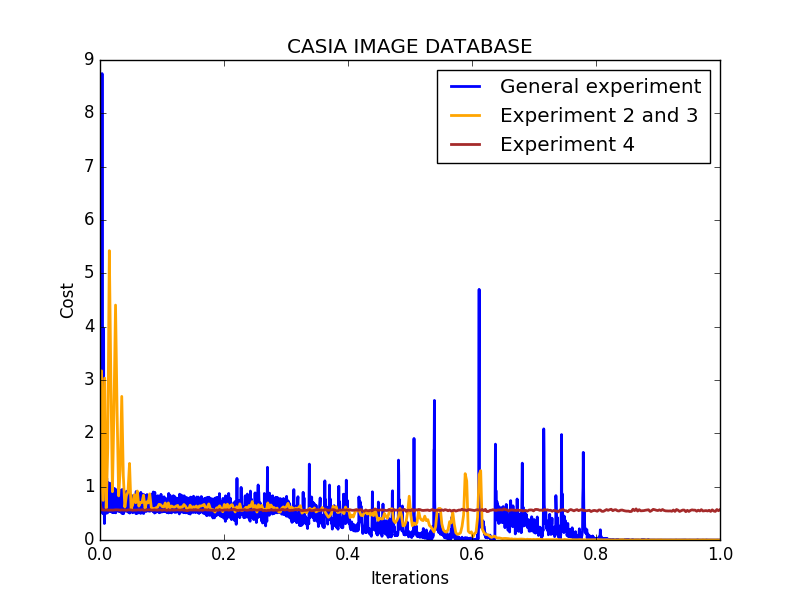
\includegraphics[width=0.48\textwidth]{images/images_ejecucion1/CASIA_im_experiments_cost_2.png} \label{fig:casia-ejec1_cost}  }
\subfigure[Error]{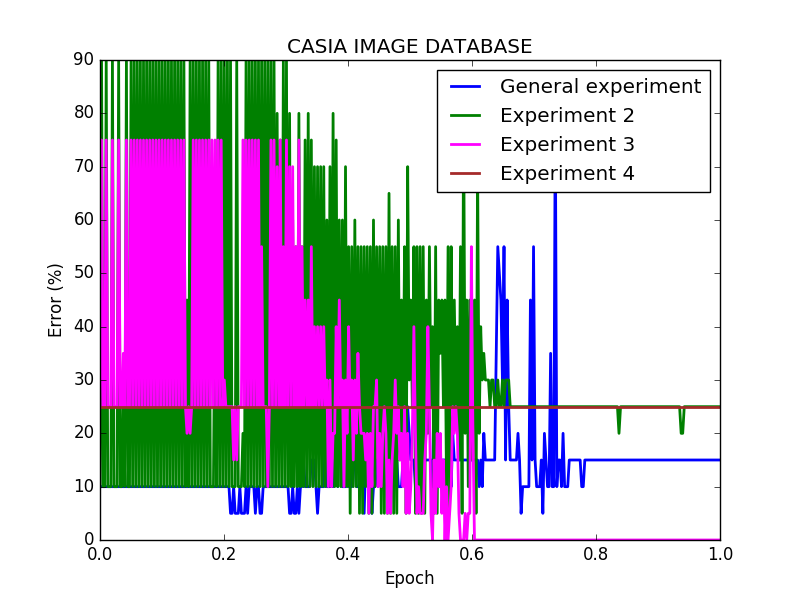
\includegraphics[width=0.48\textwidth]{images/images_ejecucion1/CASIA_im_experiments_error.png} \label{fig:casia-ejec1_error} }
\caption{Cost at training (a) and Error at validation (b) for general experiment when CASIA image database has been used.}
\label{fig:casia-ejec1}
\end{figure}

\begin{figure}[htb]
\centering
\subfigure[Cost]{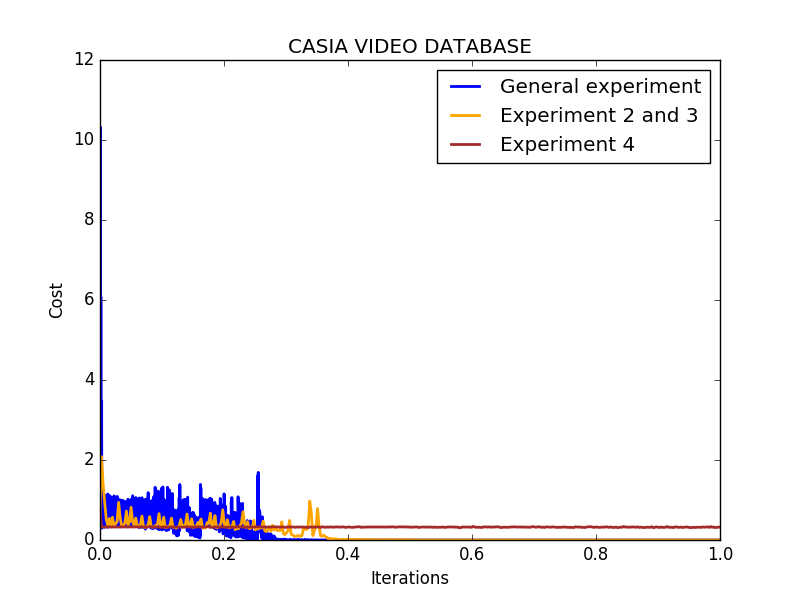
\includegraphics[width=0.48\textwidth]{images/images_ejecucion1/CASIA_vid_experiments_cost_2.png} \label{fig:casia-vid-ejec1_cost}  }
\subfigure[Error]{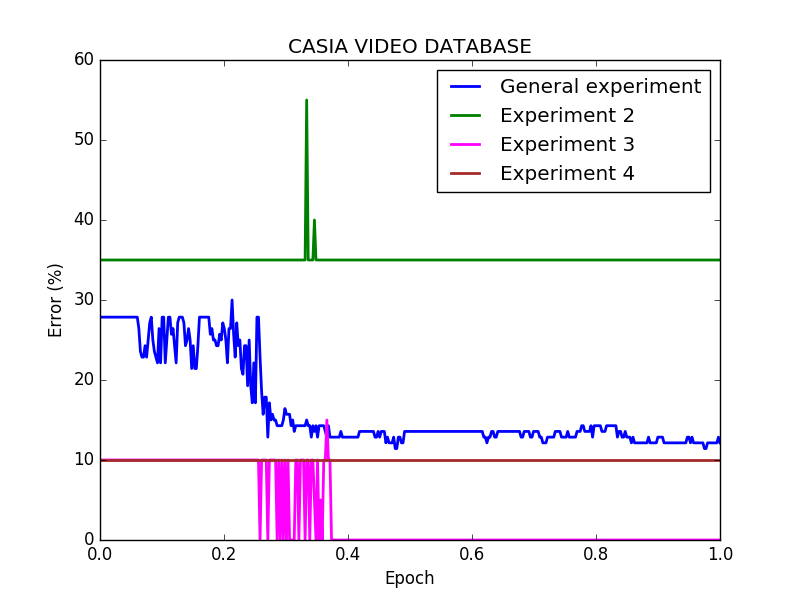
\includegraphics[width=0.48\textwidth]{images/images_ejecucion1/CASIA_vid_experiments_error.png} \label{fig:casia-vid-ejec1_error} }
\caption{Cost at training (a) and Error at validation (b) for general experiment when CASIA video database has been used.}
 \label{fig:casiavid-ejec1}
\end{figure}

\begin{figure}[htb]
\centering
\subfigure[Cost]{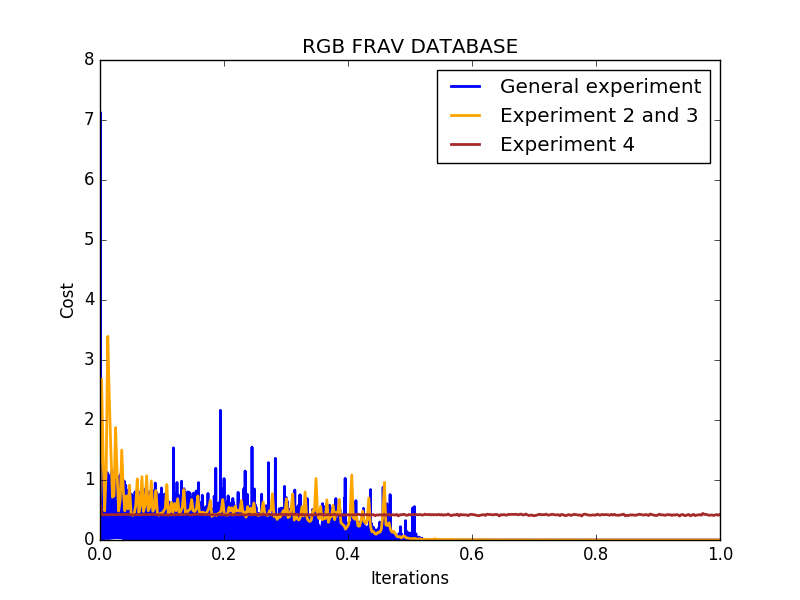
\includegraphics[width=0.48\textwidth]{images/images_ejecucion1/FRAV_experiments_cost_2.png} \label{fig:FRAV-ejec1_cost}  }
\subfigure[Error]{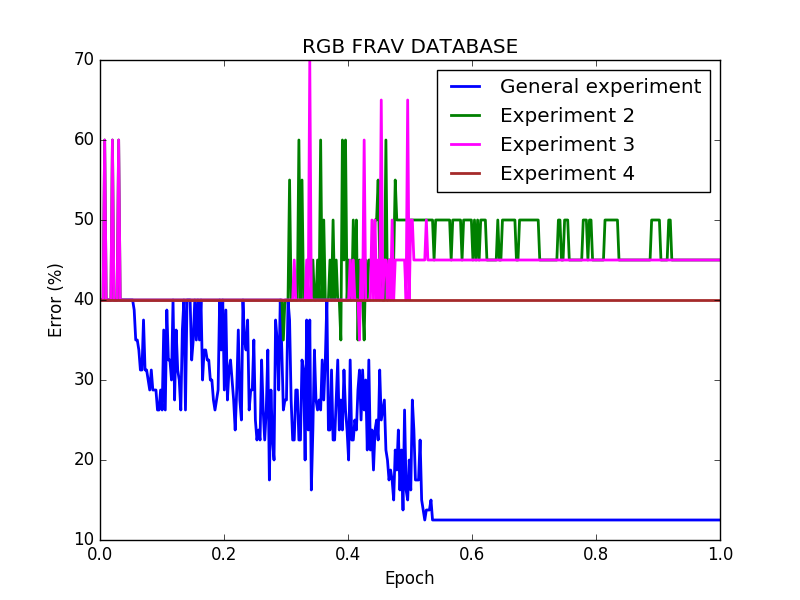
\includegraphics[width=0.48\textwidth]{images/images_ejecucion1/FRAV_experiments_error.png} \label{fig:FRAV-ejec1_error} }
\caption{Cost at training (a) and Error at validation (b) for general experiment when RGB FRAV database has been used.}
\label{fig:frav-ejec1}
\end{figure}

\clearpage

\begin{figure}[htb]
\centering
\subfigure[Cost]{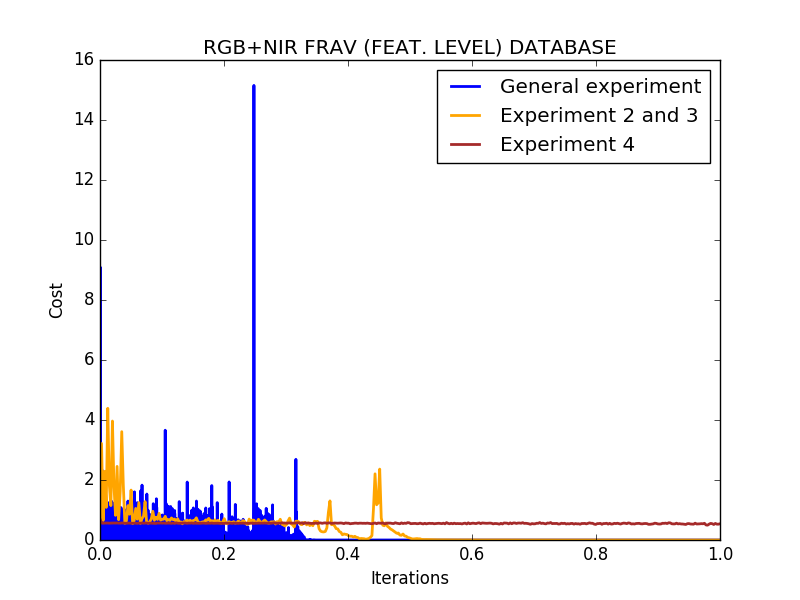
\includegraphics[width=0.48\textwidth]{images/images_ejecucion1/FRAV_FEAT_experiments_cost_2.png} \label{fig:FRAV_FEAT-ejec1_cost}  }
\subfigure[Error]{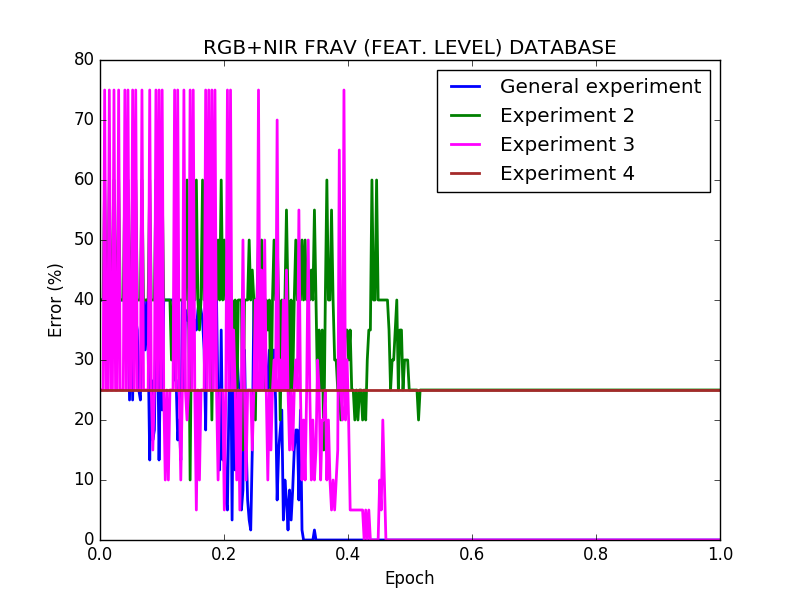
\includegraphics[width=0.48\textwidth]{images/images_ejecucion1/FRAV_FEAT_experiments_error.png} \label{fig:FRAV_FEAT-ejec1_error} }
\caption{Cost at training (a) and Error at validation (b) for general experiment when RGB+NIR (feature level) FRAV database has been used.}
\label{fig:frav_imagelevel-ejec1}
\end{figure}

\begin{figure}[htb]
\centering
\subfigure[RGB Cost]{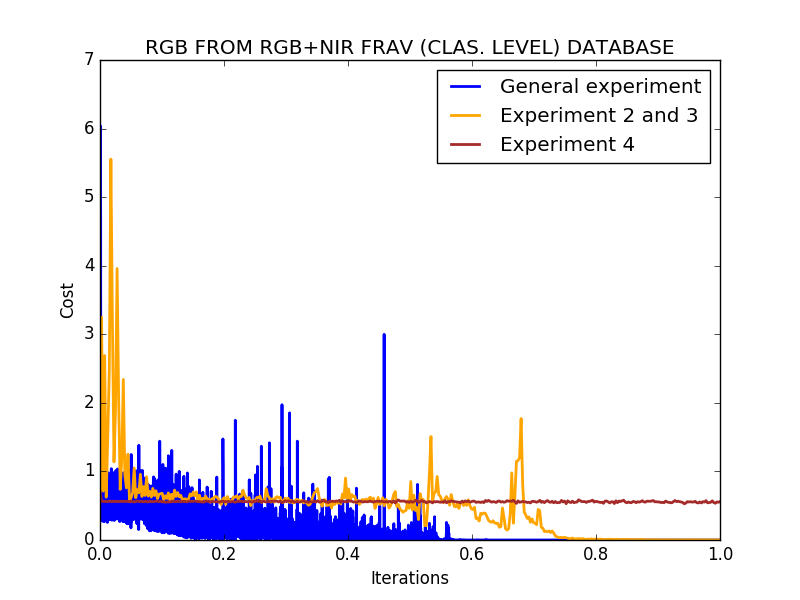
\includegraphics[width=0.48\textwidth]{images/images_ejecucion1/RGB_FRAV_CLAS_experiments_cost_2.png} \label{fig:RGB_FRAV_CLAS-ejec1_cost}  }
\subfigure[RGB Error]{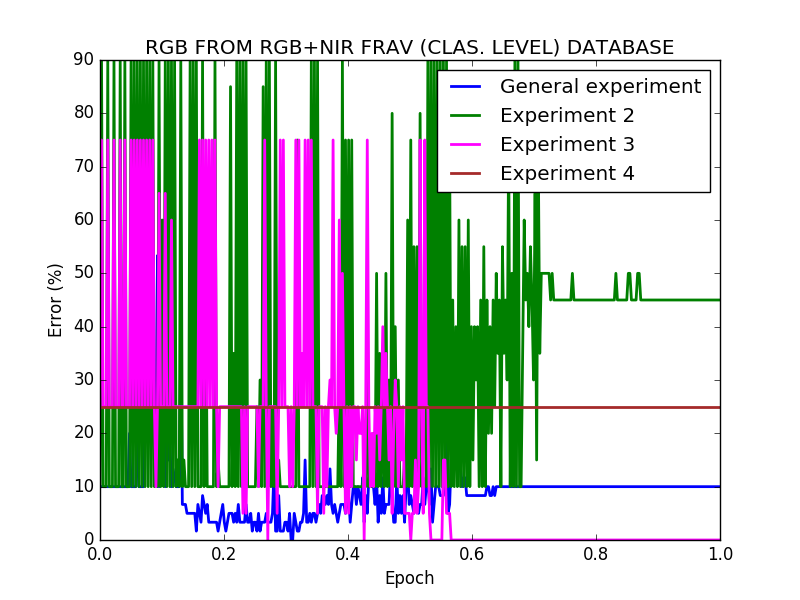
\includegraphics[width=0.45\textwidth]{images/images_ejecucion1/RGB_FRAV_CLAS_experiments_error.png} \label{fig:RGB_FRAV_CLAS-ejec1_error} }

\subfigure[NIR Cost]{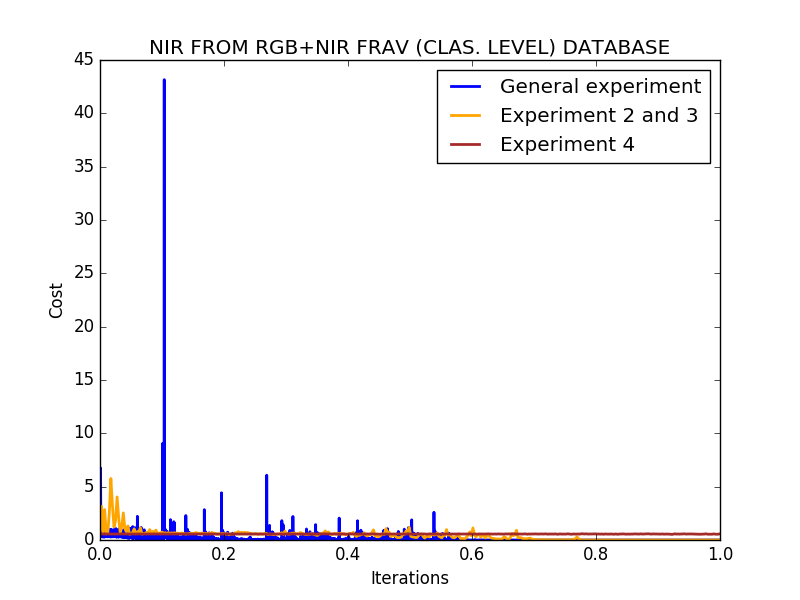
\includegraphics[width=0.48\textwidth]{images/images_ejecucion1/NIR_FRAV_CLAS_experiments_cost_2.png} \label{fig:NIR_FRAV_CLAS-ejec1_cost}  }
\subfigure[NIR Error]{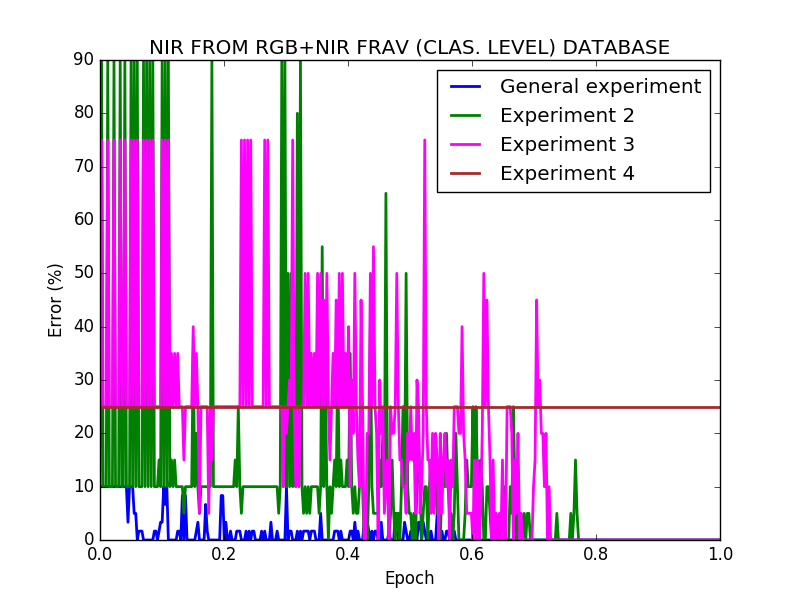
\includegraphics[width=0.45\textwidth]{images/images_ejecucion1/NIR_FRAV_CLAS_experiments_error.png} \label{fig:NIR_FRAV_CLAS-ejec1_error} }

\caption{RGB Cost at training (a) and Error at validation (b), NIR Cost at training (c) and Error at validation (d) for general experiment when RGB+NIR (classification level) FRAV database has been used.}
\label{fig:frav_classlevel-ejec1}
\end{figure}

\begin{figure}[htb]
\centering
\subfigure[Cost]{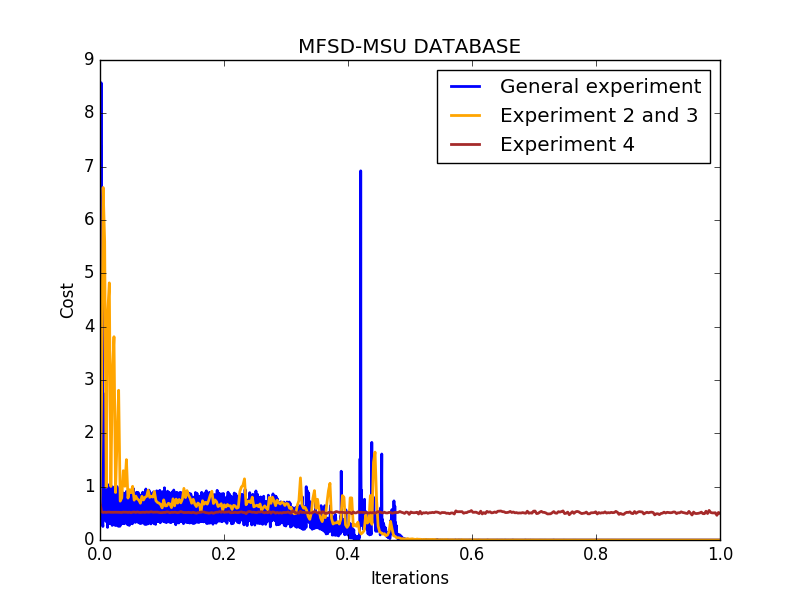
\includegraphics[width=0.48\textwidth]{images/images_ejecucion1/MFSD_experiments_cost_2.png} \label{fig:mfsd-ejec1_cost}  }
\subfigure[Error]{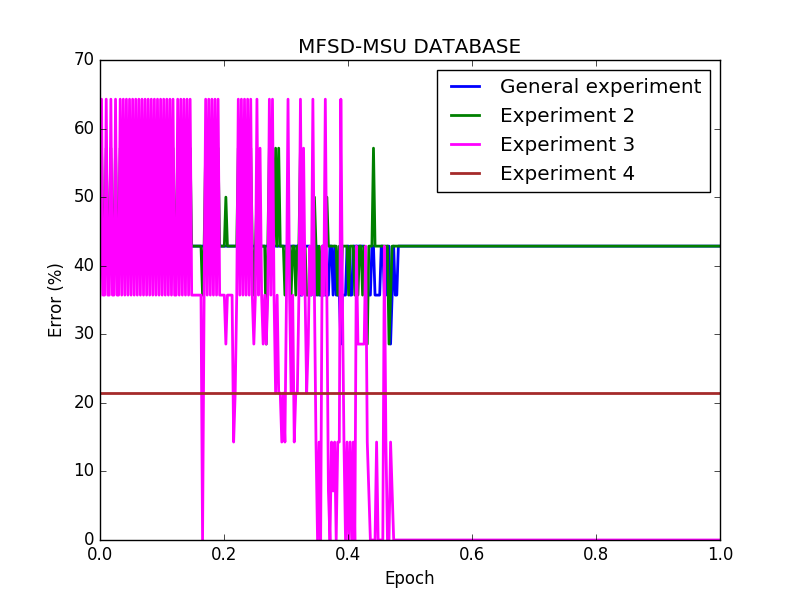
\includegraphics[width=0.48\textwidth]{images/images_ejecucion1/MFSD_experiments_error.png} \label{fig:mfsd-ejec1_error} }
\caption{Cost at training (a) and Error at validation (b) for general experiment when MFSD-MSU database has been used.}
 \label{fig:mfsd-ejec1}
\end{figure}


%In figure \ref{fig:frav-ejec1} are represented the validation error and training cost of each experiment with RGB FRAV database. RGB+NIR FRAV database results are represented in figure \ref{fig:frav_imagelevel-ejec1}. CASIA image database experiments are represented in figure  \ref{fig:casia-ejec1}, CASIA video database is represented in figure \ref{fig:casiavid-ejec1}. In figure \ref{fig:mfsd-ejec1} are represented results of MFSD-MSU database.\\


From the general experiment, can be seen that the cost converges in low values, the validation error converges (from 10\% error to very low values near to 0\% error) for all databases except for MFSD-MSU database as could be seen in figure \ref{fig:mfsd-ejec1} which means that the generalization is not correct. \\

From Experiment 2, would expect that the training and validation processes converges without oscillations and in less epochs, but because of the unbalanced samples, the validation results are worsen.\\

From Experiment 3 and experiment 2, overfitting would be expected. Just in Experiment 3 and with all databases except for FRAV one is obtained.\\

Decreasing the learning rate from 0.01 to 0.001 does not improve the performance as could be seen for all databases in figures \ref{fig:casia-ejec1}, \ref{fig:casiavid-ejec1}, \ref{fig:frav-ejec1}, \ref{fig:frav_imagelevel-ejec1}, \ref{fig:frav_classlevel-ejec1} and \ref{fig:mfsd-ejec1}. The  training curve should converge with more epochs, but the training and validation error is constant.\\

In table \ref{table-ej1} could be seen the positive and negatives rates obtained for each database when the general experiment (the fist one described) has been tested. The result obtained with RGB+NIR FRAV database is the best because just 3 samples have been misclassified from 140 images. In general, classification is not bag. The database whose samples are misclassified in a big amount is CASIA videos but the total number of samples is much bigger too.\\

\begin{table}[htb]
\centering
\begin{tabular}{c|c|c|c|c|c|}
\cline{2-6}
                                                                        & \cellcolor[HTML]{ECF4FF}\begin{tabular}[c]{@{}c@{}}SVM\\ Optima C\end{tabular} & \cellcolor[HTML]{ECF4FF}TP & \cellcolor[HTML]{ECF4FF}TN & \cellcolor[HTML]{ECF4FF}FP & \cellcolor[HTML]{ECF4FF}FN \\ \hline
\multicolumn{1}{|c|}{\cellcolor[HTML]{ECF4FF}RGB FRAV}                  & 0.05                                                                           & 136                        & 24                         & 11                         & 9                          \\ \hline
\multicolumn{1}{|c|}{\cellcolor[HTML]{ECF4FF}RGB+NIR FRAV (feat level)} & 0.1                                                                            & 113                        & 24                         & 1                          & 2                          \\ \hline
\multicolumn{1}{|c|}{\cellcolor[HTML]{ECF4FF}CASIA images}              & 5                                                                              & 9                          & 2                          & 0                          & 9                          \\ \hline
\multicolumn{1}{|c|}{\cellcolor[HTML]{ECF4FF}CASIA videos}              & 0.1                                                                            & 478                        & 75                         & 105                        & 62                         \\ \hline
\multicolumn{1}{|c|}{\cellcolor[HTML]{ECF4FF}MFSD-MSU}                  & 10                                                                             & 19                         & 1                          & 8                          & 0                          \\ \hline
\end{tabular}
\caption{TP, FP, TN and FN obtained with each database.}
\label{table-ej1}
\end{table}


The conclusion is the needed of a balanced database, at least to do this experiment. In which the number of class 0 samples are the same that the number of class 1 samples, because the network would not learn in the same way if in some cases the number of samples of  attack class is four times than the number of samples of class 1, just predicting 0 would have 25\% accuracy, and having less than 5 samples in validation or testing is not a good generalizer (2 samples in class 0 MFSD database).

\section{Final experiment}\label{sec:Final_archi} %Used in ejecucion 2
In this section, the last, and the most relevant experiment is described.\\

The architecture used for this experiment is the same as the used in \ref{subsec:ejecucion1}, the learning rate, the classifier used at training and the batch size are the same too.\\

All the databases are utilized. Samples distribution  is described in table \ref{Samples_distribution}, the same utilized as in \ref{subssec:ejec1_database}.\\

The difference between this experiment and the realized in \ref{sec:experiments_ejec1} is the classification task.\\

Each database has been trained and validated individually. The best model obtained at validation is saved for testing, for each database. Features obtained at the output of the Neural Network best model are used to fed each classifier for training (with training samples), validating (with validation samples) and testing (with testing samples).\\

Classifiers are trained with the features of the training samples. The best model of the classifier is selected depending on the features obtained of validation samples and the test is realized with the features of the test samples.\\


%\subsection{Architecture}
%The neural network is composed by five convolutional layers: the first and second convolutional layers (CL1 and CL2) , whose kernel sizes are 11x11 and 3x3 respectively, are followed by a local response normalization layer and a max pool layer whose size is 2x2. The third convolutional layer (CL3), with a kernel size of 3x3 , the next layer is a convolutional one (CL4) of size 3x3 followed by a max-pool layer whose size is 2x2. The next two layers are Dropouts layers (DL1 and DL2) with 4096 neurons. The next layer us a Fully-connected layer (FL) with 4096 neurons at the input and 2000 layers at the output.\\

%The activation function used in each layer is the ReLu. The weights have been initialized pseudo-randomly (a random initialization that could be repeated selecting the same seed) with a Gaussian distribution and the bias has been initialized with 1.\\

%It has been used the minibatch Stochastic Gradient Descend and in the training, the used classifier, is the logistic regression.\\

%The learning rate is fixed at a 0.01 value and a bath size of 20, except when the MFSD database is used, in this case, the batch size is 14.

%\subsection{Database}
%The dataset used in this experiment is the same as used in the previous architecture, the described in section \ref{subssec:ejec1_database}, but also, RGB+NIR FRAV database added in classification level is going to be used.\\

%The sample distribution is the same, which is summarized in table table \ref{Samples_distribution}. There is just one row for RGB+NIR FRAV database because the sample distribution is the same independently of when the are concatenate.\\

%Two classes has been used, class 0: the real users class and class 1: the attacks class.

%\subsection{Classification}
%For testing some classifiers has been utilized, and they are fed by the output of the convolutional neural network last layer, the Fully-connected layer.\\

The classifiers used to classify the features of the output of the CNN and get the results are the SVM (with RBF and linear kernel), KNN, Decision Tree and logistic regression. Also, PCA and LDA techniques has been used with each classifier separately to reduce the dimensionality of the features.\\

The classifiers, before use them, has been personalize to each and particular time (for each database and if LDA or PCA is used). For that, cross validation has been used, more concretely, the \textit{cros\_val\_Score()} function from sklearn has used with 10 folders:
\begin{itemize}
\item For SMV classifier, the C parameter has been searched among the following values: 0.001, 0.005, 0.01, 0.05, 0.1, 0.5, 1, 2, 3, 5 and 10.
\item For KNN classifier, the number of neighbours (K) has been searched among the following values: 2, 4, 6, 8, 10, 12, 14, 16, 18, 20, 22, 24, 26, 28 and 30.
\item For Deep Trees classifier, the depth of the tree has been searches among the following values: 2, 4, 6, 8, 10, 12, 14, 16, 18, 20, 22, 24, 26, 28 and 30.
\item For PCA, the number of components has been found in a range of 3 to 5000, in 3 to 3 steps.
\item For LDA, the number of components has been found in a range of 1 to the length of the characteristic vector in 10 to 10 steps.
\end{itemize}

%With the purpose of having a more general results, all the training, validation and testing (with the classification) processes have been repeated three times, those times are differentiated among them in the seed if the pseudo-randomized initialization of the weights.\\
\clearpage
